%
% Repaso de conceptos de teoría musical grega
\section{A música en Grecia}
%
Para escoitar e comprender ben a música dos diferentes períodos da cultura grega, debemos coñecer as principais características ou trazos que a definen. Coñecer as características, axuda a diferenciar a música de diferentes culturas, épocas, civilizacións e, asimesmo, será de utilidade á hora de completar a ficha de audición. Repasaremos aquí os aspectos básicos.
%
\subsection*{Fundamentos da teoría musical grega}\label{fundamentos}
%
Le con atención as características que definen os fundamentos da teoría musical grega e trata de identificalos nas audicións.
\begin{multicols}{2}
    \begin{enumerate}[1)]
    \item
    A música grega era \textbf{principalmente monódica}: o acompañamento instrumental, non implica harmonía ou polifonía na música grega
    \item
    Empregaba \textbf{notación alfabética}:  diferente segundo se tratase de música vocal ou instrumental
    \item
    Inicialmente emprega \textbf{ritmo libre} axustado á prosodia do texto; música e verso van unidos. Posteriormente, aparecen os \textbf{pés métricos} que se basan na duración longa ou curta das sílabas, sendo os máis comúns: \textit{Yambo}, \textit{Troqueo}, \textit{Anapesto}, \textit{Dáctilo}, (...)
    \item
    Emprega \textbf{Métrica} rica e complicada
    \item
    A \textbf{melodía} responde á idea do \textit{nomos} (lei), semellante a unha especie de patrón, esquema ou norma que rixe o sistema de composición
    \item
    O sistema musical grego é \textbf{modal}, baseado no uso do \textit{tetracordo} descendente de 4 notas
    \item
    Os \textbf{modos gregos}, están definidos polos \textit{tetracordos} e segundo a posición destes reciben un nome ou outro, que ven definido pola colocación dos \textit{semitonos} (e a súa relación interválica) e non polas notas que empregan. Os principais son:
        \begin{itemize}
            \item
            \textit{tetracordo} \textit{dórico} (T T S) = \textbf{modo dórico}, corresponde á oitava Mi-Mi
            \item
            \textit{tetracordo} \textit{frixio} (T S T) = \textbf{modo frixio}, corresponde á oitava Re-Re
            \item
            \textit{tetracordo} \textit{lidio} (S T T) = \textbf{modo lidio}, corresponde á oitava Dó-Dó
            \item
            \textbf{Modo mixolidio}, non emprega dous \textit{tetracordos} iguais = oitava Si-Si
        \end{itemize}
    \item
    Os sons a partir dos cales se organiza o sistema musical grego, parten de relacións numéricas sinxelas definidas por Pitágoras a partir do \textit{monocordio}
    \item
    O sistema musical grego, recibe o nome de \textbf{\textit{sistema diatónico teleion}} que comprende 2 oitavas.
    \item
    A escala Mi-Mi é a máis importante: coincide coa afinación (das cordas) da \textit{kithara} e coñecíase tamén co nome de "Harmonía"
    \end{enumerate}
\end{multicols}
%
\subsection*{Os tres himnos de Mesomedes de Creta}
%
Escoita os tres himnos de Mesomedes de Creta (\textit{Invocación a Calíope e Apolo}, \textit{Himno a Helio} e \textit{Himno a Némesis}) que podes atopar na {\href{https://open.spotify.com/playlist/19fWZwUGX6rDo0bejNcWGE?si=1c00d5ff65b24678}{\textcolor{blue}{lista de audicións}}} de Spotify e trata de identificar as principais características da teoría musical grega que se indican no punto anterior.
\par
%
\subsubsection*{O \textit{Himno a Némesis}}
%
Este himno de Mesomedes de Creta, é un dos catro que conservan notación musical antiga sobre o texto; a figura \ref{nemesis-himno} é unha transcrición a notación actual do himno.
%
\begin{figure}[htp]
    \centering
	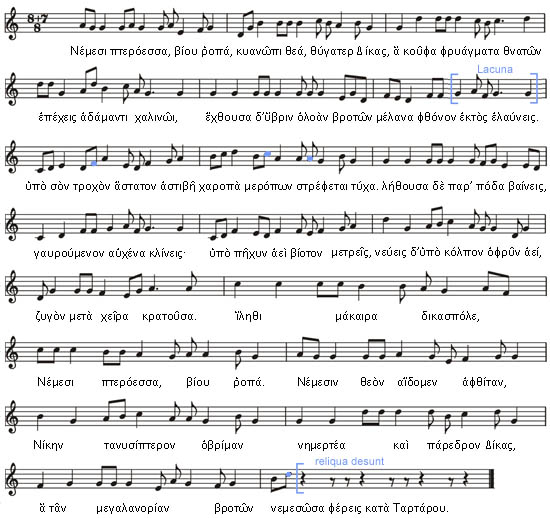
\includegraphics[scale=0.80]{images/mes-hnem.jpg}
	\caption{Exemplo do himno a némesis}
	\label{nemesis-himno}
	\end{figure}
%
\begin{ejercicio}[Comentario resumo do \textit{Himno a Némesis}]
Fai un breve comentario sobre o himno, seguindo os puntos anteriores.
% ESPACIO PARA REDACTAR O COMENTARIO DA AUDICIÓN
        \vspace*{3.3cm}
\end{ejercicio}
 
